% \documentclass[handout]{beamer}
\documentclass{beamer}

\mode<presentation>
{
  \usetheme{ANLBlue}
  % \usefonttheme[onlymath]{serif}
  % \usetheme{Singapore}
  % \usetheme{Warsaw}
  % \usetheme{Malmoe}
  % \useinnertheme{circles}
  % \useoutertheme{infolines}
  % \useinnertheme{rounded}

  \setbeamercovered{transparent=20}
}

\usepackage[english]{babel}
\usepackage[latin1]{inputenc}
\usepackage{alltt,listings,multirow,ulem,siunitx}
\usepackage[absolute,overlay]{textpos}
\TPGrid{1}{1}
\usepackage{pdfpages}
\usepackage{multimedia}
\usepackage{multicol}
\newcommand\hmmax{0}
\newcommand\bmmax{0}
\usepackage{bm}
\usepackage{comment}

% font definitions, try \usepackage{ae} instead of the following
% three lines if you don't like this look
\usepackage{mathptmx}
\usepackage[scaled=.90]{helvet}
% \usepackage{courier}
\usepackage[T1]{fontenc}
\usepackage{tikz}
\usetikzlibrary{decorations.pathreplacing}
\usetikzlibrary{shadows,arrows,shapes.misc,shapes.arrows,shapes.multipart,arrows,decorations.pathmorphing,backgrounds,positioning,fit,petri,calc,shadows,chains,matrix}


% \usepackage{pgfpages}
% \pgfpagesuselayout{4 on 1}[a4paper,landscape,border shrink=5mm]

\usepackage{JedMacros}

\newcommand{\timeR}{t_{\mathrm{R}}}
\newcommand{\timeW}{t_{\mathrm{W}}}
\newcommand{\mglevel}{\ensuremath{\ell}}
\newcommand{\mglevelcp}{\ensuremath{\mglevel_{\mathrm{cp}}}}
\newcommand{\mglevelcoarse}{\ensuremath{\mglevel_{\mathrm{coarse}}}}
\newcommand{\mglevelfine}{\ensuremath{\mglevel_{\mathrm{fine}}}}

%solution and residual
\newcommand{\vx}{\ensuremath{x}}
\newcommand{\vc}{\ensuremath{\hat{x}}}
\newcommand{\vr}{\ensuremath{r}}
\newcommand{\vb}{\ensuremath{b}}

%operators
\newcommand{\vA}{\ensuremath{A}}
\newcommand{\vP}{\ensuremath{I_H^h}}
\newcommand{\vS}{\ensuremath{S}}
\newcommand{\vR}{\ensuremath{I_h^H}}
\newcommand{\vI}{\ensuremath{\hat I_h^H}}
\newcommand{\vV}{\ensuremath{\mathbf{V}}}
\newcommand{\vF}{\ensuremath{F}}
\newcommand{\vtau}{\ensuremath{\mathbf{\tau}}}


\title{Vectorization, communication aggregation, and reuse in stochastic and temporal dimensions}
\author{Jed Brown \\ \url{jedbrown@mcs.anl.gov}}

% - Use the \inst command only if there are several affiliations.
% - Keep it simple, no one is interested in your street address.
\institute
{
  Mathematics and Computer Science Division \\ Argonne National Laboratory
}

\date{Exascale Math Workshop, 2013-08-21}

% This is only inserted into the PDF information catalog. Can be left
% out.
\subject{Talks}


% If you have a file called "university-logo-filename.xxx", where xxx
% is a graphic format that can be processed by latex or pdflatex,
% resp., then you can add a logo as follows:

% \pgfdeclareimage[height=0.5cm]{university-logo}{university-logo-filename}
% \logo{\pgfuseimage{university-logo}}



% Delete this, if you do not want the table of contents to pop up at
% the beginning of each subsection:
% \AtBeginSubsection[]
% {
% \begin{frame}<beamer>
%   \frametitle{Outline}
%   \tableofcontents[currentsection,currentsubsection]
% \end{frame}
% }

\AtBeginSection[]
{
  \begin{frame}<beamer>
    \frametitle{Outline}
    \tableofcontents[currentsection]
  \end{frame}
}

% If you wish to uncover everything in a step-wise fashion, uncomment
% the following command:

% \beamerdefaultoverlayspecification{<+->}

\begin{document}
\lstset{language=C}
\normalem

\begin{frame}
  \titlepage
\end{frame}


\begin{frame}{Premise}
  \begin{itemize}
  \item Transformative science and engineering
    \begin{itemize}
    \item Better analysis
      \begin{itemize}
      \item design optimization with uncertainty
      \item risk minimization, rare events, experimental design
      \item diverse data sources with multiphysics
      \end{itemize}
    \item Human time scales: real-time, interactivity, field study guidance
    \end{itemize}
  \item Traditional abstractions are comfortable, but not optimal
    \begin{itemize}
    \item Parallelism of components without holistic view
    \item Attempts to optimize lead to ``tunnel vision''
    \item Want end-to-end efficiency at desired turn-around time
    \item Eternal trade-off: total memory use vs parallelism/critical path length
    \end{itemize}
  \item Transparency in formerly-opaque abstractions enables composition that produces more effective optimization
  \item More regularity beyond the spatial domain
    % Minimize negative log posterior, initial convergence gives
    % information about thickness of the tails of the posterior.
  \end{itemize}
\end{frame}

\begin{frame}{Beyond the spatial domain: The stack is deep}
  \begin{itemize}
  \item forward model: transient PDE model
    \begin{itemize}
    \item $u(t,x; p)$ with parameters $p$ known (initial/boundary data, coefficients, \ldots)
    \end{itemize}
  \item forward model with uncertainty: stochastic representation of incompletely-modeled processes
    \begin{itemize}
    \item $u(t,x,\mathfrak z; p)$ with noise $\mathfrak z$ in stochastic space
    \end{itemize}
  \item Design optimization with uncertainty
    \begin{itemize}
    \item $\min_p \int_{\mathfrak z} f(u(t,x,\mathfrak z,p) ) $
    \end{itemize}
  \item data assimilation: infer $p$ from sparse observations $d_0$ with noise $\mathfrak y$
    \begin{equation*}
    \hat p(t,x,d,d_0) = \argmin_p \int_{\mathfrak y} \int_{\mathfrak z} \norm{d(u(t,x,\mathfrak z,p) + \mathfrak y) - d_0}^2 + \mathrm{Prior}(p)
  \end{equation*}
  \item optimal experimental design: choose ``affordable'' sparse observations $d$ to minimize risk in the data assimilation problem over a region of parameter/model space
    \begin{equation*}
      \hat d = \argmin_d \int_p \norm{\hat p(t,x,d,d_0(p)) - p} + \mathrm{cost}(d)
    \end{equation*}
  \item ``collocation'' (decoupled ensemble) vs. Galerkin (coupled)
  \end{itemize}
\end{frame}

% \begin{frame}{Principles}
%   \begin{itemize}
%   \item Eternal trade-off: total memory use and parallelism/critical path length
%   \item Memory locality: cache reuse/sharing, GPU shared memory, NUMA
%     \begin{itemize}
%     \item Get the maximum use out of data before we retire it from cache
%     \end{itemize}
%   \item Exploitable regularity
%     \begin{itemize}
%     \item Vectorization: packed SSE/AVX/QPX, avoid warp divergence
%     \item Coalesced loads, prefetchable streams
%     \item Ability to share cache between threads
%     \item Avoid contention in case of overlapped writes
%     \end{itemize}
%   \end{itemize}
% \end{frame}

\begin{frame}{The quest for exploitable regularity}
  \begin{columns}
    \begin{column}{0.5\textwidth}
      \begin{block}{Spatial domain}
        \begin{itemize}
        \item Complex geometry
        \item Non-smooth transient features (e.g., fracture, corners, shocks)
        \item Free boundaries
        \item Boundary conditions
        \item Spatial adaptivity
        \item Only distribute spatial domain
        \item Pipeline length is costly
        \end{itemize} 
      \end{block}
    \end{column}
    \begin{column}{0.5\textwidth}
      \begin{block}{Temporal/stochastic domain}
        \begin{itemize}
        \item Simple/no geometry
        \item Internally smoother (branch jumps rare)
        \item Little or no boundary conditions (initial conditions)
        \item Global time steps for stiff problems (but local for hyperbolic)
        \item Data size up to proportional to entire simulation
        \end{itemize}      
      \end{block}
    \end{column}
  \end{columns}
  \begin{itemize}
  \item<2> \alert{Aggregate:} vectorize, amortize communication; same total work
  \item<2> \alert{Synergy:} mutually-beneficial reuse/accelerated convergence
  \end{itemize}
\end{frame}

\begin{frame}{Example: $s$-step methods in 3D}
  \includegraphics[width=\textwidth]{figures/SStepEfficiency.pdf}
  \begin{itemize}
  \item Amortizing message latency is most important for strong-scaling
  \item $s$-step methods have high overhead for small subdomains
  \item Limited choice of preconditioners (none optimal)
  \end{itemize}
\end{frame}

% \begin{frame}{Example: space-time methods (multilevel SDC/Parareal)}
%   \includegraphics[width=0.9\textwidth]{figures/EmmettMinionPFASSTCost.png}
%   \begin{itemize}
%   \item PFASST algorithm (Emmett and Minion, 2013)
%   \item Zero-latency messages (cf. performance model of $s$-step)
%   \item Spectral Deferred Correction: iterative, converges to IRK (Gauss, Radau, \ldots)
%   \item Stiff problems use implicit basic integrator (synchronizing on spatial communicator)
%   \end{itemize}
% \end{frame}

% \begin{frame}{Merging Implicit Runge-Kutta with Multigrid}
%   \begin{itemize}
%   \item Expand view to space-time Implicit RK problem
%   \item PFASST is a line smoother (accurate solve in spatial domain)
%   %\item PFASST uses finest-possible decomposition in time (latency-intolerant)
%   % \item Status quo for IRK with direct methods:
%   %   \begin{itemize}
%   %   \item Modified Newton using spectral decomposition of Butcher matrix $A$
%   %   \end{itemize}
%   \item What about: chunky space-time domain with space-time smoother?
%   \item Aggregate
%     \begin{itemize}
%     \item Amortize or pipeline communication over stages (no overhead)
%     \item Vectorize nonlinear residual over stages
%     \end{itemize}
%   \item Synergy
%     \begin{itemize}
%     \item Reuse point/cell Jacobian in smoother for all stages (point-modified Newton, cf. Implicit RK)
%     \item Frozen $\tau$ for parabolic problems (Brandt and Greenwald, \emph{Parabolic multigrid revisited}, 1991)
%     \item Selectively multiplicative in time (Vandewalle and Horton, \emph{Fourier mode analysis of the multigrid waveform relaxation and time-parallel multigrid methods}, 1995)
%     \item Block/recycling Krylov acceleration
%     \end{itemize}
%   \end{itemize}
% \end{frame}

% \begin{frame}{Merging stochastic with multigrid}
%   \begin{itemize}
%   \item 
%   \end{itemize}
% \end{frame}

\begin{frame}{A notion of coupling rank}
  \begin{itemize}
  \item ``Full space'' (spatial, temporal, parameters, stochastic, \ldots)
  \end{itemize}
  \begin{figure}
    \centering
    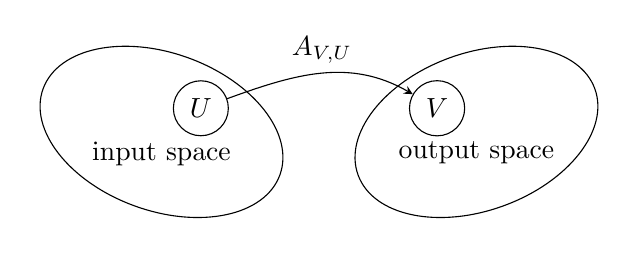
\begin{tikzpicture}
      [>=stealth]
      \draw (0,0) circle [x radius=1.6, y radius=1, rotate=-20] node[below] {input space};
      \draw (4,0) circle [x radius=1.6, y radius=1, rotate=20] node[below] {output space};
      % \draw (0.5,0.5) circle [radius=.3] node{$U$};
      % \draw (3.6,0.6) circle [x radius=.2, y radius=.3] node{$V$};
      \node[circle,radius=.3,draw] (U) at (0.5,0.3) {$U$};
      \node[circle,x radius=.2,y radius=.3,draw] (V) at (3.5,0.3) {$V$};
      \draw[->] (U) to[out=20,in=150] node[above] {$A_{V,U}$} (V);
    \end{tikzpicture}
  \end{figure}
  \begin{itemize}
  \item $A_{V,U}$: dependence of solution in subdomain $V$ on data from subdomain $U$
  \item Essential rank $k$ of $A_{V,U}$ is number of singular values greater than chosen relative tolerance
  \item Crude lower bound: at least $k$ units of information must be communicated from $U$ to $V$
  \item Parallel distribution: high-rank couplings should be ``nearby''
  \end{itemize}
\end{frame}

\begin{frame}{Implication of essential coupling rank for anisotropy}
  Anisotropic diffusion:
  \begin{equation*}
    -\nabla\cdot (\kappa \nabla u) = f, \qquad \kappa =
    \begin{pmatrix}
      \epsilon & 0 \\ 0 & 1
    \end{pmatrix}
  \end{equation*}
  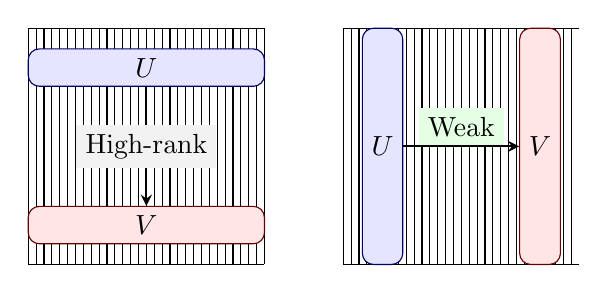
\begin{tikzpicture}[
    >=stealth,
    uset/.style={draw=blue!40!black,fill=blue!10,rounded corners},
    vset/.style={draw=red!40!black,fill=red!10,rounded corners}
    ]
    \draw (0,0) grid[xstep=0.1,ystep=3] (3,3);
    \draw (4,0) grid[xstep=0.1,ystep=3] (7,3);
    \node[uset,minimum width=3cm] (Uunaligned) at (1.5,2.5) {$U$};
    \node[vset,minimum width=3cm] (Vunaligned) at (1.5,0.5) {$V$};
    \node[uset,minimum height=3cm] (Ualigned) at (4.5,1.5) {$U$};
    \node[vset,minimum height=3cm] (Valigned) at (6.5,1.5) {$V$};
    \draw[->,thick] (Uunaligned) -- node[fill=gray!10] {High-rank} (Vunaligned);
    \draw[->,thick] (Ualigned) -- node[fill=green!10,above] {Weak} (Valigned);
  \end{tikzpicture}
  \begin{itemize}
  \item Surrogate for space-time-stochastic, 1-way and 2-way coupling
  \item Identical distribution for input and output spaces is common.
  \item The $k$ items of data can be communicated in different ways:
    \begin{itemize}
    \item Increasingly-large subdomains at greater distance (tree-code)
    \item Interaction through coarse grid (multigrid, fast multipole)
    \end{itemize}
  \item Space-time: causality cone steeper in space than time
  \end{itemize}
\end{frame}

% \begin{frame}{Essential rank in space-time}
%   \begin{itemize}
%   \item Higher rank coupling in time than space
%     \begin{itemize}
%     \item Hyperbolic equation $\Delta x = \lambda_{\max} \Delta t$:
%       causality cone is steeper in time than space (equivalent for
%       fastest wave at CFL 1).
%     \item Parabolic: Green's function decays faster in space than in time (depends on $\Delta t$)
%     \end{itemize}
%   \end{itemize}
% \end{frame}

\begin{frame}{Ramifications and research priorities}
  \begin{itemize}
  \item No need to focus on strict independence
    \begin{itemize}
    \item We will communicate globally anyway
    \item Choose distributions to make long-distance (in space/time/stochastic) communications low-rank
    \item ``Treecode-to-FMM'' transformations to further exploit low-rank
    \end{itemize}
  \item Exploit structure to aggregate communication and vectorize
  \item Raise temporal and stochastic dimensions to first-class
    \begin{itemize}
    \item Algorithms in full space, map to space-time computation
    \end{itemize}
  \item Adaptive recognition of reusability/synergistic structure
  \item Load balancing due to adaptive spatio-temporal-stochastic reuse
  \item Evolution of software interfaces
    \begin{itemize}
    \item Nuanced problem structure
    \item Reusable components that do less than ``solve'' the sub-problem
    \end{itemize}
  \item Extend analysis to ``full-space'' methods
  \item Programming tools
    \begin{itemize}
    \item Unintrusive manipulation of logical vector length
    \item Support for judicious use of cross-lane operations
    \item Asynchronous and aggregated communication
    \end{itemize}
  \end{itemize}
\end{frame}

\end{document}
